\documentclass[11pt,a4paper]{article}

\usepackage{amsmath,amssymb,amsthm}
\usepackage{mathtools}
\usepackage{bm}
\usepackage{enumerate}
\usepackage{hyperref}
\usepackage{cleveref}
\usepackage[margin=1in]{geometry}
\usepackage{tikz}
\usetikzlibrary{arrows.meta,calc,decorations.pathreplacing,fit,positioning}
\usepackage{pgfplots}
\pgfplotsset{compat=1.18}
\usepackage{tcolorbox}
\usepackage{booktabs}

% Theorem environments
\newtheorem{theorem}{Theorem}[section]
\newtheorem{lemma}[theorem]{Lemma}
\newtheorem{proposition}[theorem]{Proposition}
\newtheorem{corollary}[theorem]{Corollary}
\theoremstyle{definition}
\newtheorem{definition}[theorem]{Definition}
\newtheorem{example}[theorem]{Example}
\newtheorem{remark}[theorem]{Remark}

% Notation shortcuts
\newcommand{\E}{\mathbb{E}}
\newcommand{\Var}{\mathrm{Var}}
\newcommand{\Normal}{\mathcal{N}}
\newcommand{\given}{\,|\,}
\newcommand{\btheta}{\boldsymbol{\theta}}
\newcommand{\bmu}{\boldsymbol{\mu}}
\newcommand{\bpsi}{\boldsymbol{\psi}}
\DeclareMathOperator{\CE}{CE}
\DeclareMathOperator{\RDU}{RDU}
\DeclareMathOperator{\tr}{tr}

% Highlight box for key results
\newtcolorbox{keyresult}[1][]{
    colback=blue!5!white,
    colframe=blue!50!black,
    fonttitle=\bfseries,
    title={#1},
}

\title{Over-Determined CE Priors:\\
Model-Agnostic Observable-Space Prior Specification\\
via the Pullback Measure}
\author{Technical Note}
\date{February 2026}

\begin{document}

\maketitle

\begin{abstract}
The companion note on the Jacobian correction derives the induced prior
$p_{\btheta}(\btheta) = p_{\mathbf{Y}}(\mathbf{g}(\btheta)) \, |\!\det
J_{\mathbf{g}}(\btheta)|$ for the case where the mapping
$\mathbf{g}: \mathbb{R}^k \to \mathbb{R}^k$ is a square diffeomorphism ---
the same number of observable quantities (CEs) as model parameters. This note
extends the framework to the \emph{over-determined} case where there are more
observables than parameters: $\mathbf{g}: \mathbb{R}^k \to \mathbb{R}^n$
with $k < n$. The image of $\mathbf{g}$ is a $k$-dimensional manifold
embedded in $n$-dimensional CE space. The correct induced prior replaces the
determinant with the \emph{Gram determinant}:
$p_{\btheta}(\btheta) = p_{\mathbf{Y}}(\mathbf{g}(\btheta))
\sqrt{\det(J^\top\! J)}$, where $J$ is the $n \times k$ Jacobian. This
generalization is not merely a mathematical curiosity --- it enables
\textbf{model-agnostic} CE-space priors that work unchanged across utility
specifications of different dimensionality, and it provides a natural
Occam's razor for model comparison.
\end{abstract}

\tableofcontents
\newpage


%==============================================================================
\section{The Problem: Mismatched Dimensions}
\label{sec:problem}
%==============================================================================

\subsection{Where This Arises}

Consider a researcher who specifies prior beliefs about the certainty
equivalents (CEs) of two reference lotteries:
\begin{equation}
    \CE_1 \sim \Normal(27, 25), \qquad \CE_2 \sim \Normal(22, 25)
\end{equation}
These beliefs are stated in dollar terms and are cognitively natural: ``I think
the CE of lottery $L_1$ is about \$27 $\pm$ \$5.''

Now suppose the researcher estimates two different utility models on the same
data:
\begin{enumerate}
    \item \textbf{Expo-Power EUT} with 2 parameters $(r, \beta)$. The mapping
    $\mathbf{g}_{\text{EP}}: \mathbb{R}^2 \to \mathbb{R}^2$ is square.
    \item \textbf{CRRA EUT} with 1 parameter $(r)$. The mapping
    $\mathbf{g}_{\text{CRRA}}: \mathbb{R}^1 \to \mathbb{R}^2$ maps into a
    1-dimensional \emph{curve} in 2D CE space.
\end{enumerate}

For the Expo-Power model, the Jacobian correction from the companion note
applies directly: $|\!\det J|$ of the $2 \times 2$ Jacobian. But for CRRA,
$J$ is $2 \times 1$ --- not square --- and $\det J$ is not defined.

\subsection{The Na\"ive Reaction}

The natural first response is: ``You can't use 2 CEs to specify a prior for 1
parameter. The Jacobian correction requires a square matrix. Pick just 1 CE, or
use a model with 2 parameters.''

This reaction is understandable but wrong. The correct framework is the
\emph{pullback measure} from differential geometry, which generalizes the
Jacobian correction to non-square mappings. The key insight is that the square
case is a special instance of a more general volume-element construction.

\subsection{Why This Matters}

Before diving into the mathematics, here is why the over-determined case is
worth developing:

\begin{enumerate}
    \item \textbf{Model-agnostic priors.} The researcher's beliefs about CEs
    do not depend on which utility function will be estimated. The same 2D
    CE prior should work for both CRRA and Expo-Power, with the model
    determining which subset of CE space is reachable.

    \item \textbf{Fair model comparison.} If the same CE prior is used
    across models, Bayes factors for model comparison reflect only how well
    each model fits the data, not artifacts of incompatible prior
    specifications.

    \item \textbf{Natural Occam's razor.} The CRRA model can only access a
    1D curve in the 2D CE prior. The Expo-Power model can access the full 2D
    plane. This automatically penalizes the more flexible model unless the
    data genuinely require the extra dimension --- exactly the Bayesian
    Occam's razor.

    \item \textbf{Robustness.} Using more CEs than parameters provides
    over-identification: the prior is anchored by multiple observable
    constraints rather than a single one.
\end{enumerate}


%==============================================================================
\section{Review: The Square Case}
\label{sec:square}
%==============================================================================

We briefly recall the result from the companion note, to establish notation
for the generalization.

When $\mathbf{g}: \mathbb{R}^k \to \mathbb{R}^k$ is a smooth injection (a
diffeomorphism onto its image), the induced prior on $\btheta \in \mathbb{R}^k$
from a density $p_{\mathbf{Y}}$ on $\mathbf{Y} = \mathbf{g}(\btheta) \in
\mathbb{R}^k$ is:
\begin{equation}
    \label{eq:square}
    p_{\btheta}(\btheta) = p_{\mathbf{Y}}\!\big(\mathbf{g}(\btheta)\big) \;
    \big|\!\det J_{\mathbf{g}}(\btheta)\big|
\end{equation}
where $J_{\mathbf{g}}$ is the $k \times k$ Jacobian matrix with entries
$(J)_{ij} = \partial g_i / \partial \theta_j$.

The factor $|\!\det J|$ is the local volume scaling: a small $k$-dimensional
box of volume $dV_\theta$ in parameter space maps to a parallelotope of volume
$|\!\det J| \cdot dV_\theta$ in $Y$-space. The probability of landing in the
image parallelotope under $p_{\mathbf{Y}}$ must equal the probability of
landing in the original box under $p_{\btheta}$.


%==============================================================================
\section{The Over-Determined Case: Derivation}
\label{sec:derivation}
%==============================================================================

\subsection{Setup}

Let $\btheta \in \mathbb{R}^k$ be the parameter vector and
$\mathbf{Y} = \mathbf{g}(\btheta) \in \mathbb{R}^n$ the CE vector, with
$k < n$. The image $\mathcal{M} = \mathbf{g}(\mathbb{R}^k)$ is a
$k$-dimensional manifold (a ``surface'') embedded in $\mathbb{R}^n$.

We specify a density $p_{\mathbf{Y}}(\mathbf{y})$ on all of $\mathbb{R}^n$
--- for instance, a product of independent normals on $(\CE_1, \CE_2)$. The
question is: what density does this induce on $\btheta$?

\subsection{The Core Issue: What Replaces \texorpdfstring{$|\!\det J|$}{|det J|}?}

The square-case derivation used the fact that a small $k$-cube in
$\btheta$-space maps to a $k$-dimensional parallelotope in $Y$-space, and the
volume ratio is $|\!\det J|$. When $k < n$, the Jacobian $J$ is $n \times k$
(more rows than columns), and $\det J$ is undefined for non-square matrices.

But the \emph{volume} of the image parallelotope is still perfectly well
defined. We just need the right formula for the $k$-dimensional volume of a
parallelotope embedded in $\mathbb{R}^n$.

\subsection{Volume of a Parallelotope in Higher Dimensions}

Consider $k$ vectors $\mathbf{v}_1, \ldots, \mathbf{v}_k \in \mathbb{R}^n$.
The $k$-dimensional volume of the parallelotope they span is:
\begin{equation}
    \label{eq:gram_volume}
    \text{vol}_k = \sqrt{\det(G)}
    \qquad \text{where} \quad G_{ij} = \mathbf{v}_i \cdot \mathbf{v}_j
\end{equation}
Here $G$ is the \emph{Gram matrix} of the vectors. If we stack the vectors as
columns of a matrix $V = [\mathbf{v}_1 \mid \cdots \mid \mathbf{v}_k]$ (which
is $n \times k$), then $G = V^\top V$ and:
\begin{equation}
    \text{vol}_k = \sqrt{\det(V^\top V)}
\end{equation}

\begin{remark}[Connection to the square case]
When $n = k$, the matrix $V$ is square and
$\det(V^\top V) = (\det V)^2 = |\!\det V|^2$, so
$\sqrt{\det(V^\top V)} = |\!\det V|$. The Gram determinant reduces to the
ordinary absolute determinant.
\end{remark}

\subsection{Applying to the Jacobian}

The columns of the Jacobian $J = J_{\mathbf{g}}(\btheta)$ are exactly the
images of the coordinate directions $\mathbf{e}_1, \ldots, \mathbf{e}_k$
under the linearization of $\mathbf{g}$ at $\btheta$. A small cube in
$\btheta$-space with sides $d\theta_1, \ldots, d\theta_k$ maps to a
$k$-dimensional parallelotope spanned by
$J\mathbf{e}_1 \cdot d\theta_1, \ldots, J\mathbf{e}_k \cdot d\theta_k$,
i.e., by the columns of $J$ scaled by $d\theta_j$.

The $k$-dimensional volume of this image parallelotope is:
\begin{equation}
    dV_{\mathcal{M}} = \sqrt{\det(J^\top J)} \; d\theta_1 \cdots d\theta_k
\end{equation}

This is the \emph{area element} (or volume element) of the embedded manifold
$\mathcal{M}$ in the parameterization $\btheta$.

\subsection{The Induced Density}

The probability conservation argument is identical to the square case. The
probability in a small $\btheta$-box must equal the probability that
$\mathbf{Y}$ lands in the image parallelotope on $\mathcal{M}$:
\begin{equation}
    p_{\btheta}(\btheta) \; dV_\theta
    = p_{\mathbf{Y}}\!\big(\mathbf{g}(\btheta)\big) \; dV_{\mathcal{M}}
    = p_{\mathbf{Y}}\!\big(\mathbf{g}(\btheta)\big) \;
    \sqrt{\det(J^\top J)} \; dV_\theta
\end{equation}
Canceling $dV_\theta$:

\begin{keyresult}[The Pullback Prior (Over-Determined Case)]
\begin{equation}
    \label{eq:pullback}
    \boxed{
    p_{\btheta}(\btheta) = p_{\mathbf{Y}}\!\big(\mathbf{g}(\btheta)\big) \;
    \sqrt{\det\!\big(J_{\mathbf{g}}(\btheta)^\top \,
    J_{\mathbf{g}}(\btheta)\big)}
    }
\end{equation}
where $J_{\mathbf{g}}$ is the $n \times k$ Jacobian of $\mathbf{g}$.
\end{keyresult}

\begin{remark}[Nomenclature]
This construction is the \emph{pullback} of the ambient measure
$p_{\mathbf{Y}} \, d\mathbf{y}$ by the embedding $\mathbf{g}$. The factor
$\sqrt{\det(J^\top J)}$ is variously called the \emph{Gram determinant}, the
\emph{area element}, or the \emph{metric determinant} of the induced
Riemannian metric on $\mathcal{M}$.
\end{remark}

\subsection{Formal Statement}

\begin{theorem}[Pullback measure for immersions]
\label{thm:pullback}
Let $\mathbf{g}: \Omega \subset \mathbb{R}^k \to \mathbb{R}^n$ be a $C^1$
immersion ($k \leq n$, $\text{rank}\, J_{\mathbf{g}} = k$ everywhere) that is
injective on $\Omega$. Let $p_{\mathbf{Y}}: \mathbb{R}^n \to [0, \infty)$ be a
Lebesgue-measurable density on $\mathbb{R}^n$. Then the pullback density on
$\Omega$ is:
\begin{equation}
    p_{\btheta}(\btheta) = p_{\mathbf{Y}}\!\big(\mathbf{g}(\btheta)\big) \;
    \sqrt{\det\!\big(J_{\mathbf{g}}(\btheta)^\top \,
    J_{\mathbf{g}}(\btheta)\big)}
\end{equation}
This $p_{\btheta}$ is a well-defined (possibly unnormalized) density on
$\Omega$ that satisfies:
\begin{equation}
    \int_\Omega f(\btheta) \, p_{\btheta}(\btheta) \, d\btheta
    = \int_{\mathcal{M}} f\!\big(\mathbf{g}^{-1}(\mathbf{y})\big) \,
    p_{\mathbf{Y}}(\mathbf{y}) \, d\sigma(\mathbf{y})
\end{equation}
for any integrable $f$, where $d\sigma$ is the $k$-dimensional Hausdorff
measure (surface area measure) on $\mathcal{M} = \mathbf{g}(\Omega)$.
\end{theorem}

\begin{proof}[Proof sketch]
This is the area formula from geometric measure theory (see, e.g., Evans and
Gariepy, \emph{Measure Theory and Fine Properties of Functions}, Theorem 3.9).
The area formula states that for a Lipschitz map $\mathbf{g}: \mathbb{R}^k
\to \mathbb{R}^n$ and a non-negative measurable function $h$:
\begin{equation}
    \int_{\mathbb{R}^k} h(\btheta) \,
    \sqrt{\det(J_{\mathbf{g}}^\top J_{\mathbf{g}})} \, d\btheta
    = \int_{\mathbb{R}^n} \sum_{\btheta \in \mathbf{g}^{-1}(\mathbf{y})}
    h(\btheta) \; d\mathcal{H}^k(\mathbf{y})
\end{equation}
When $\mathbf{g}$ is injective, the sum on the right has at most one term, and
the result follows by taking $h(\btheta) = f(\btheta) \,
p_{\mathbf{Y}}(\mathbf{g}(\btheta))$.
\end{proof}


%==============================================================================
\section{Geometric Picture}
\label{sec:geometry}
%==============================================================================

\subsection{The Manifold in CE Space}

When $k < n$, the model constrains the joint CE values to lie on a
$k$-dimensional surface $\mathcal{M}$ in $n$-dimensional CE space. Different
utility specifications produce different surfaces.

\begin{figure}[ht]
\centering
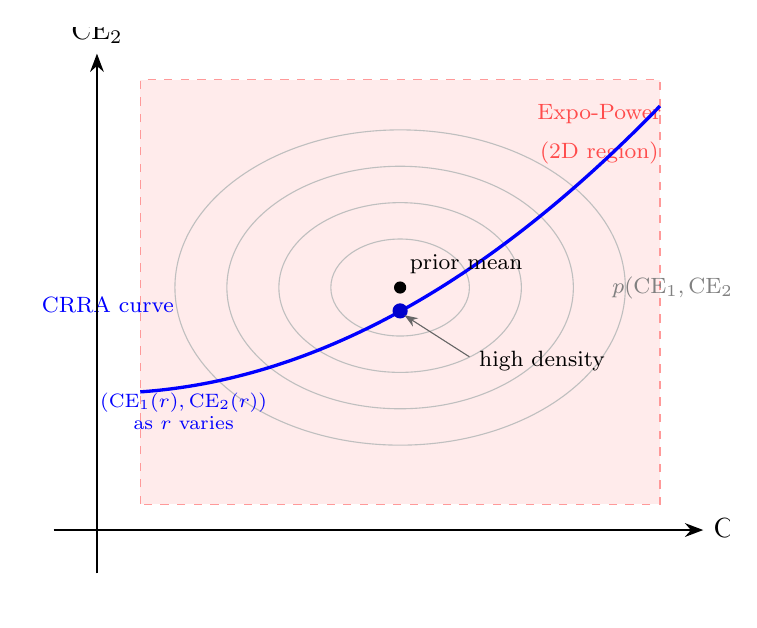
\begin{tikzpicture}[>=Stealth, scale=1.1]
    % Clip to plot region
    \clip (-0.8,-0.8) rectangle (7.3,5.8);

    % Expo-Power region (background, drawn first)
    \fill[red!8] (0.5,0.3) rectangle (6.5,5.2);
    \draw[red!40, dashed] (0.5,0.3) rectangle (6.5,5.2);
    \node[red!70, font=\footnotesize] at (5.8,4.8) {Expo-Power};
    \node[red!70, font=\footnotesize] at (5.8,4.35) {(2D region)};

    % 2D Normal prior (contours)
    \foreach \s in {0.8, 1.4, 2.0, 2.6} {
        \draw[gray!50, thin] (3.5,2.8) ellipse ({\s} and {0.7*\s});
    }
    \node[gray] at (6.7,2.8) {\footnotesize $p(\CE_1, \CE_2)$};

    % CRRA curve — a gentle arc through the contours
    \draw[very thick, blue, smooth, domain=0.5:6.5, samples=80]
        plot (\x, {0.08*(\x-3.5)^2 + 0.55*\x + 0.6});
    \node[blue, above left] at (1.0,2.4) {\footnotesize CRRA curve};
    \node[blue, below, font=\scriptsize, text width=2.8cm, align=center]
        at (1.0,1.7) {$(\CE_1(r), \CE_2(r))$\\as $r$ varies};

    % Axes (drawn on top)
    \draw[->, thick] (-0.5,0) -- (7,0) node[right] {$\CE_1$};
    \draw[->, thick] (0,-0.5) -- (0,5.5) node[above] {$\CE_2$};

    % Mark the prior mean
    \fill[black] (3.5,2.8) circle (2pt);
    \node[above right, font=\footnotesize] at (3.5,2.85) {prior mean};

    % Mark where CRRA curve is near prior mean
    \fill[blue!80!black] (3.5,2.53) circle (2.5pt);
    \draw[->, thin, black!60] (4.3,2.0) -- (3.55,2.48);
    \node[right, font=\footnotesize] at (4.3,1.95) {high density};
\end{tikzpicture}
\caption{%
    A 2D Normal prior on $(\CE_1, \CE_2)$ (gray contours). The Expo-Power
    model can reach any point in the 2D plane (light red region). The CRRA
    model is restricted to a 1D curve (blue). The induced prior on $r$
    concentrates where the CRRA curve passes near the prior mean. Regions of
    the curve far from the prior center receive low density --- the prior
    penalizes parameter values whose implied CEs are far from the
    researcher's beliefs.
}
\label{fig:manifold}
\end{figure}

\subsection{What the Gram Determinant Measures}

In the square case, $|\!\det J|$ measures how the mapping scales
$k$-dimensional volumes. In the over-determined case,
$\sqrt{\det(J^\top J)}$ measures the same thing, but the ``volume'' is the
$k$-dimensional area of the image parallelotope as it sits inside
$\mathbb{R}^n$.

The geometric intuition is simplest for $k = 1$, $n = 2$:

\begin{itemize}
    \item $\btheta = r$ is a scalar parameter.
    \item $\mathbf{g}(r) = (\CE_1(r), \CE_2(r))$ traces a curve in the
    $(\CE_1, \CE_2)$ plane.
    \item $J = \begin{pmatrix} d\CE_1/dr \\ d\CE_2/dr \end{pmatrix}$ is a
    $2 \times 1$ column vector.
    \item $J^\top J = (d\CE_1/dr)^2 + (d\CE_2/dr)^2$ is a $1 \times 1$
    matrix (a scalar).
    \item $\sqrt{\det(J^\top J)} = \sqrt{(d\CE_1/dr)^2 + (d\CE_2/dr)^2}
    = \|\mathbf{g}'(r)\|$ --- the \emph{speed} of the curve.
\end{itemize}

\begin{keyresult}[The 1-in-2 case]
For a single parameter $r$ and two CEs:
\begin{equation}
    \label{eq:1in2}
    p_r(r) = p_{\CE_1, \CE_2}\!\big(\CE_1(r),\, \CE_2(r)\big) \;
    \left\|\frac{d\mathbf{g}}{dr}\right\|
    = p_{\CE_1, \CE_2}\!\big(\CE_1(r),\, \CE_2(r)\big) \;
    \sqrt{\left(\frac{d\CE_1}{dr}\right)^{\!2}
    + \left(\frac{d\CE_2}{dr}\right)^{\!2}}
\end{equation}
\end{keyresult}

\noindent
The speed $\|\mathbf{g}'(r)\|$ measures how fast the CE pair changes as $r$
varies. Where the curve moves quickly through CE space, a small $dr$ interval
sweeps out a long arc, ``collecting'' more CE-space probability. Where the
curve is nearly stationary, the same $dr$ interval covers only a short arc
and collects less probability.

\begin{figure}[ht]
\centering
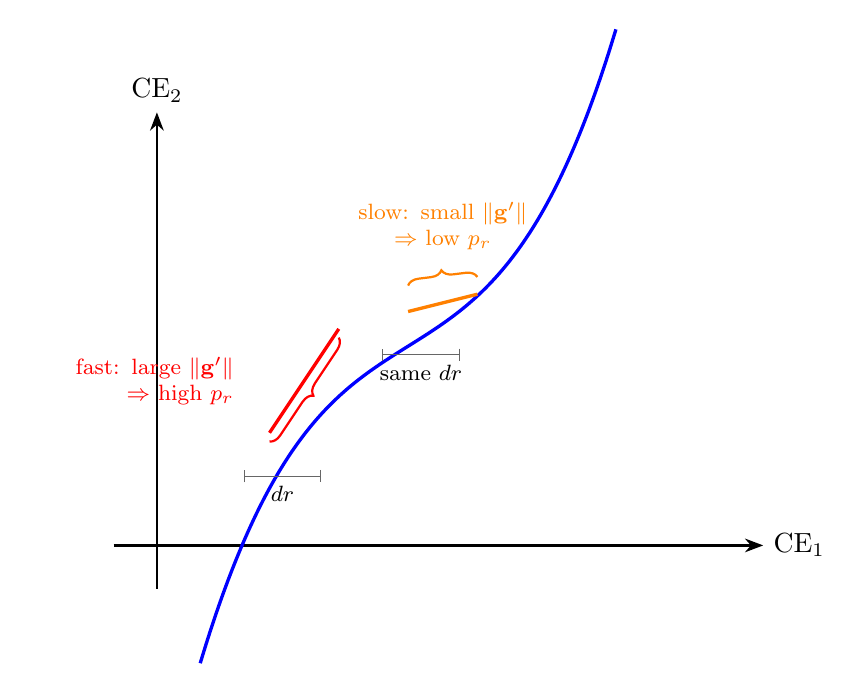
\begin{tikzpicture}[>=Stealth, scale=1.1]
    % Axes
    \draw[->, thick] (-0.5,0) -- (7,0) node[right] {$\CE_1$};
    \draw[->, thick] (0,-0.5) -- (0,5) node[above] {$\CE_2$};

    % Curve (parametric)
    \draw[very thick, blue, smooth, domain=0:6, samples=60]
        plot ({0.8*\x + 0.5}, {0.08*(\x-3)^3 + 0.5*\x + 0.8});

    % Mark a fast segment (steep slope)
    \draw[very thick, red] (1.3,1.3) -- (2.1,2.5);
    \node[red, left, font=\footnotesize, text width=2.5cm, align=right]
        at (1.0,1.9) {fast: large $\|\mathbf{g}'\|$\\$\Rightarrow$ high $p_r$};
    \draw[decorate, decoration={brace, amplitude=4pt, mirror},
          thick, red] (1.3,1.2) -- (2.1,2.4);

    % Mark a slow segment (flat slope)
    \draw[very thick, orange] (2.9,2.7) -- (3.7,2.9);
    \node[orange, above, font=\footnotesize, text width=2.5cm, align=center]
        at (3.3,3.3) {slow: small $\|\mathbf{g}'\|$\\$\Rightarrow$ low $p_r$};
    \draw[decorate, decoration={brace, amplitude=4pt},
          thick, orange] (2.9,3.0) -- (3.7,3.1);

    % dr labels
    \draw[|-|, thin, black!60] (1.0,0.8) -- (1.9,0.8);
    \node[below, font=\footnotesize] at (1.45,0.8) {$dr$};
    \draw[|-|, thin, black!60] (2.6,2.2) -- (3.5,2.2);
    \node[below, font=\footnotesize] at (3.05,2.2) {same $dr$};
\end{tikzpicture}
\caption{%
    The same increment $dr$ in parameter space produces different arc lengths
    in CE space. Where the curve is steep (fast-moving), $\|\mathbf{g}'(r)\|$
    is large and the induced prior density $p_r(r)$ is high. Where the curve
    is flat (slow-moving), the density is low. This is the 1D-in-2D analog of
    the interval-stretching picture from the companion note.
}
\label{fig:speed}
\end{figure}


%==============================================================================
\section{Why the Square Determinant Fails and the Gram Determinant Works}
\label{sec:why}
%==============================================================================

This section addresses the conceptual question head-on: why can't we just use
the standard $|\!\det J|$ formula, and what changes when $J$ is non-square?

\subsection{The Square Case Revisited}

In the square case ($k = n$), a small $k$-cube in $\btheta$-space maps to a
$k$-dimensional parallelotope in a $k$-dimensional ambient space. The
parallelotope's volume is $|\!\det J| \cdot dV_\theta$, and the density
$p_{\mathbf{Y}}$ assigns probability to this volume in the obvious way:
$p_{\mathbf{Y}}(\mathbf{y}) \cdot dV_Y$.

The key assumption, implicit in the companion note, is that the parallelotope
is full-dimensional in the ambient space --- it has nonzero $k$-dimensional
Lebesgue measure. This is automatic when $k = n$ and $\det J \neq 0$.

\subsection{Why the Determinant Is Undefined for Non-Square Matrices}

When $k < n$, the Jacobian $J$ is $n \times k$ with more rows than columns.
The determinant is only defined for square matrices because it measures the
signed volume of a parallelepiped in a space of the \emph{same} dimension as
the number of vectors. With $k$ vectors in $\mathbb{R}^n$, the parallelepiped
is $k$-dimensional, sitting inside an $n$-dimensional space. There is no
$n$-dimensional volume to measure --- the parallelepiped has zero
$n$-dimensional Lebesgue measure.

This is not a failure of the method; it reflects a genuine geometric fact: the
image $\mathcal{M}$ is a lower-dimensional surface in $\mathbb{R}^n$, and
$n$-dimensional Lebesgue measure assigns zero probability to it. The prior
$p_{\mathbf{Y}}$ has all its mass spread over the full $n$-dimensional space,
and the manifold $\mathcal{M}$ occupies zero volume in that space.

\subsection{What the Gram Determinant Does}

The resolution is to measure $k$-dimensional volume \emph{within the manifold}
rather than $n$-dimensional volume in the ambient space. The Gram matrix
$G = J^\top J$ is $k \times k$ (always square!), and $\sqrt{\det G}$ gives the
$k$-dimensional volume of the image parallelotope.

\begin{keyresult}[Why the Gram matrix is always square]
Regardless of the dimensions $k$ and $n$:
\begin{equation}
    J \text{ is } n \times k, \qquad
    J^\top \text{ is } k \times n, \qquad
    J^\top J \text{ is } k \times k
\end{equation}
The Gram matrix $J^\top J$ is always $k \times k$, so its determinant is
always well-defined.
\end{keyresult}

\subsection{The Unified Formula}

We can state a single formula that works for all cases:

\begin{keyresult}[Unified Jacobian Correction]
For $\mathbf{g}: \mathbb{R}^k \to \mathbb{R}^n$ with $k \leq n$ and
$\text{rank}\, J_{\mathbf{g}} = k$:
\begin{equation}
    \label{eq:unified}
    p_{\btheta}(\btheta) = p_{\mathbf{Y}}\!\big(\mathbf{g}(\btheta)\big) \;
    \sqrt{\det\!\big(J_{\mathbf{g}}^\top \, J_{\mathbf{g}}\big)}
\end{equation}
\begin{itemize}
    \item When $k = n$: $\sqrt{\det(J^\top J)} = |\!\det J|$ (the companion
    note's formula).
    \item When $k < n$: $\sqrt{\det(J^\top J)}$ is the $k$-dimensional area
    element (the new formula).
\end{itemize}
\end{keyresult}

Equation~\eqref{eq:unified} subsumes the square case. All results from the
companion note --- forward-only evaluation, automatic differentiation, the
BHM extension --- carry over unchanged.


%==============================================================================
\section{Detailed Example: CRRA with Two CEs}
\label{sec:crra}
%==============================================================================

\subsection{Setup}

Consider CRRA utility $u(x) = x^{1-r}/(1-r)$ with a single parameter $r$.
We specify two reference lotteries:
\begin{align}
    L_1 &: \text{prizes } (10, 30, 50) \text{ with probs } (1/3, 1/3, 1/3)
    & \text{EV} &= 30 \\
    L_2 &: \text{prizes } (10, 30, 50) \text{ with probs } (1/2, 3/10, 1/5)
    & \text{EV} &= 23
\end{align}

Under CRRA (EUT with linear probability weighting), the CE of a lottery with
prizes $x_1 \leq x_2 \leq x_3$ and probabilities $p_1, p_2, p_3$ is:
\begin{equation}
    \CE(r) = \left[p_1 x_1^{1-r} + p_2 x_2^{1-r} + p_3 x_3^{1-r}
    \right]^{1/(1-r)}
\end{equation}

The mapping $\mathbf{g}(r) = (\CE_1(r), \CE_2(r))$ traces a curve in the
$(\CE_1, \CE_2)$ plane.

\subsection{The Jacobian}

$J$ is $2 \times 1$:
\begin{equation}
    J = \begin{pmatrix} d\CE_1/dr \\ d\CE_2/dr \end{pmatrix}
\end{equation}

The Gram ``matrix'' is a scalar:
\begin{equation}
    J^\top J = \left(\frac{d\CE_1}{dr}\right)^{\!2}
    + \left(\frac{d\CE_2}{dr}\right)^{\!2}
\end{equation}

And the area element is:
\begin{equation}
    \sqrt{\det(J^\top J)} = \sqrt{\left(\frac{d\CE_1}{dr}\right)^{\!2}
    + \left(\frac{d\CE_2}{dr}\right)^{\!2}}
    = \left\|\frac{d\mathbf{g}}{dr}\right\|
\end{equation}

\subsection{The Induced Prior}

Specifying an independent normal prior on CEs:
\begin{equation}
    \CE_1 \sim \Normal(27, 25), \qquad \CE_2 \sim \Normal(22, 25)
\end{equation}

The induced prior on $r$ is:
\begin{equation}
    \label{eq:crra_prior}
    p_r(r) = \phi\!\left(\frac{\CE_1(r) - 27}{5}\right) \cdot \frac{1}{5}
    \;\cdot\; \phi\!\left(\frac{\CE_2(r) - 22}{5}\right) \cdot \frac{1}{5}
    \;\cdot\; \left\|\frac{d\mathbf{g}}{dr}\right\|
\end{equation}
where $\phi$ is the standard normal density.

\subsection{Interpretation}

The prior density on $r$ is high when \emph{both} of the following hold:
\begin{enumerate}
    \item The implied CEs $(\CE_1(r), \CE_2(r))$ are close to the prior means
    $(27, 22)$ --- both normal factors are large.
    \item The CE curve is moving quickly through CE space at that $r$ ---
    $\|\mathbf{g}'(r)\|$ is large.
\end{enumerate}

Condition (1) is intuitive: the prior favors parameter values whose
implied CEs match the researcher's beliefs. Condition (2) is the Jacobian
correction: it adjusts for the ``density'' of the parameterization. A region
where the curve is nearly flat (CEs barely change with $r$) receives lower
weight because many $r$ values produce essentially the same CE --- the
parameterization is ``redundant'' there.

\subsection{Computational Implementation}

In code (using JAX):
\begin{verbatim}
    def g(r):
        ce1 = crra_ce(r, prizes1, probs1)
        ce2 = crra_ce(r, prizes2, probs2)
        return jnp.array([ce1, ce2])

    J = jax.jacfwd(g)(r)          # shape (2, 1)
    gram = J.T @ J                 # shape (1, 1)
    log_area = 0.5 * jnp.log(jnp.linalg.det(gram))

    # Equivalently for k=1:
    log_area = 0.5 * jnp.log(jnp.sum(J**2))
\end{verbatim}

For the general $k < n$ case:
\begin{verbatim}
    J = jax.jacfwd(g)(theta)      # shape (n, k)
    gram = J.T @ J                 # shape (k, k)
    sign, logdet = jnp.linalg.slogdet(gram)
    log_area = 0.5 * logdet
\end{verbatim}

Note the factor of $1/2$: we need $\sqrt{\det(J^\top J)}$, so on the log
scale this is $\frac{1}{2} \log \det(J^\top J)$.


%==============================================================================
\section{Model-Agnostic Priors}
\label{sec:model_agnostic}
%==============================================================================

\subsection{The Key Insight}

The CE-space prior $p_{\mathbf{Y}}(\mathbf{y})$ encodes the researcher's
beliefs about observable quantities. These beliefs do not depend on the
parametric utility model being estimated. A statement like ``the CE of lottery
$L_1$ is about \$27 $\pm$ \$5'' is a statement about preferences, not about
whether utility is CRRA, Expo-Power, or anything else.

This means the \emph{same} CE prior can be used with different utility
models:
\begin{enumerate}
    \item For a $k$-parameter model: $\mathbf{g}: \mathbb{R}^k \to
    \mathbb{R}^n$. The induced prior uses $\sqrt{\det(J^\top J)}$ with an
    $n \times k$ Jacobian.
    \item For a $k'$-parameter model ($k' \neq k$):
    $\mathbf{g}': \mathbb{R}^{k'} \to \mathbb{R}^n$, same CE prior, different
    Jacobian dimensions.
\end{enumerate}

As long as $n \geq \max(k, k')$, the same $n$-dimensional CE prior works for
both models without any modification.

\subsection{The Hierarchy of Models}

Consider a sequence of nested utility models, all estimated with the same
data and the same $n = 3$ CE prior:

\begin{center}
\begin{tabular}{llcc}
\toprule
Model & Parameters & $k$ & Manifold dimension \\
\midrule
CRRA (EUT) & $r$ & 1 & 1D curve in $\mathbb{R}^3$ \\
CRRA (RDU, 1-param PWF) & $r, \phi$ & 2 & 2D surface in $\mathbb{R}^3$ \\
Prelec RDU & $r, \phi, \eta$ & 3 & 3D (fills $\mathbb{R}^3$) \\
\bottomrule
\end{tabular}
\end{center}

Each model accesses a different-dimensional slice of the CE prior:
\begin{itemize}
    \item CRRA sees a 1D curve: the prior concentrates on the point of that
    curve nearest the prior mean.
    \item 1-param RDU sees a 2D surface: more flexibility to match the
    prior, but still constrained.
    \item Full Prelec RDU fills 3D CE space: maximum flexibility.
\end{itemize}

The more constrained models receive a prior that is automatically more
concentrated (in parameter space), because fewer parameter values are
consistent with the CE beliefs.

\subsection{Occam's Razor for Model Comparison}

This structure provides a natural Bayesian Occam's razor. In a Bayes factor
comparison:
\begin{equation}
    \text{BF}_{12} = \frac{p(\text{data} \given M_1)}{p(\text{data} \given M_2)}
    = \frac{\int p(\text{data} \given \btheta_1, M_1) \,
    p(\btheta_1 \given M_1) \, d\btheta_1}
    {\int p(\text{data} \given \btheta_2, M_2) \,
    p(\btheta_2 \given M_2) \, d\btheta_2}
\end{equation}

The model with more parameters has a higher-dimensional integration domain.
The CE prior spreads its mass over this larger space. If the extra parameters
don't help explain the data, the additional spread is wasted --- the marginal
likelihood is diluted. This is the standard Occam's razor mechanism, but here
it operates through a \emph{shared, interpretable} prior rather than through
ad hoc parameter-space priors that may not be comparable.

The crucial feature is that the CE prior is the same object for both models.
The Bayes factor reflects genuine differences in model fit and parsimony, not
artifacts of different prior scales in incommensurable parameter spaces.


%==============================================================================
\section{Cross-Domain Priors and Data-Uninformed Parameters}
\label{sec:cross_domain}
%==============================================================================

The model-agnostic framework of the previous section considers a single prior
applied to models of different dimensionality, all operating within the
\emph{same economic domain} (e.g., risk preferences). This section extends the
framework to a more ambitious setting: a joint prior over observable quantities
from \emph{multiple economic domains} --- risk, time, and beyond --- applied to
a model and dataset that may speak to only a subset of those domains.

\subsection{The Vision: A Universal Prior over Economic Observables}

Imagine a researcher who maintains a single joint prior over a large vector of
economic observables:
\begin{equation}
    \mathbf{Y} = \big(\underbrace{\CE_1, \CE_2, \CE_3}_{\text{risk CEs}},\;
    \underbrace{\mathrm{PV}_1, \mathrm{PV}_2}_{\text{present values}},\;
    \underbrace{\mathrm{WTP}_1}_{\text{willingness to pay}},\; \ldots\big)
    \in \mathbb{R}^n
\end{equation}
This prior encodes beliefs about behavior across domains: ``the CE of lottery
$L_1$ is about \$27,'' ``the present value of \$100 received in one year is
about \$92,'' and so on. Crucially, the prior may encode \emph{cross-domain
correlations}: ``people who are more risk-averse also tend to discount the
future more heavily.''

The question is: what happens when we apply this joint prior to a model and
dataset that only address \emph{some} of these quantities?

There are three distinct cases, each with different mathematical behavior. We
treat them in order of increasing subtlety.

\subsection{Case 1: Disconnected Quantities (Zero Jacobian Rows)}

Suppose the model has parameters $\btheta = (r)$ (CRRA risk aversion only) and
the mapping $\mathbf{g}$ can compute CEs but has no mechanism to compute
present values --- there is no discount rate parameter. Then:
\begin{equation}
    \mathbf{g}(r) = \big(\CE_1(r),\; \CE_2(r),\; \CE_3(r),\;
    \underbrace{??,\; ??}_{\text{undefined}}\big)
\end{equation}
The model cannot produce values for $\mathrm{PV}_1$ or $\mathrm{PV}_2$, so
the corresponding Jacobian rows are not merely zero --- they are \emph{absent}.
There is no forward map into those dimensions.

The resolution is \textbf{marginalization}. We integrate out the unreachable
dimensions:
\begin{equation}
    \bar{p}_{\mathbf{Y}}(\CE_1, \CE_2, \CE_3)
    = \int p_{\mathbf{Y}}(\CE_1, \CE_2, \CE_3, v_1, v_2, \ldots)\;
    dv_1\, dv_2 \cdots
\end{equation}
and apply the pullback formula using the marginal prior
$\bar{p}_{\mathbf{Y}}$ and the reduced mapping
$\mathbf{g}(r) = (\CE_1(r), \CE_2(r), \CE_3(r))$.

If the prior is \textbf{independent} across domains ---
$p_{\mathbf{Y}}(\mathbf{c}, \mathbf{v}) = p_{\text{risk}}(\mathbf{c}) \cdot
p_{\text{disc}}(\mathbf{v})$ --- then the marginalization simply drops the
discounting factor:
\begin{equation}
    \bar{p}_{\mathbf{Y}}(\mathbf{c}) = p_{\text{risk}}(\mathbf{c})
\end{equation}
The disconnected quantities vanish as if they were never specified.

If the prior has \textbf{cross-correlations}, the marginalization produces a
marginal $\bar{p}_{\mathbf{Y}}(\mathbf{c})$ that differs from the standalone
risk prior. This is a real effect: the researcher's beliefs about the
relationship between risk and discounting alter the effective risk prior,
even though the model cannot compute present values. Whether this is desirable
depends on the researcher's intent.

\begin{keyresult}[Case 1: Disconnected quantities]
When the model has no forward map into certain observable dimensions, those
dimensions must be marginalized out of the joint prior. Under independence,
they drop out completely. Under cross-correlation, they shift the marginal
prior on the reachable dimensions.
\end{keyresult}

\subsection{Case 2: Data-Uninformed Parameters (The Interesting Case)}
\label{sec:data_uninformed}

Now consider a richer model with parameters
$\btheta = (r, \delta)$, where $r$ is CRRA risk aversion and $\delta$ is a
discount factor. Following Andersen, Harrison, Lau \& Rutstr\"{o}m
(2008)\footnote{Andersen, S., Harrison, G.W., Lau, M.I.\ \&
Rutstr\"{o}m, E.E.\ (2008). ``Eliciting Risk and Time Preferences.''
\textit{Econometrica}, 76(3), 583--618.}
and the subsequent literature, the present value of a future payment $M$
received at time $T$ is defined through the \emph{discounted utility}
equation:
\begin{equation}
    u(\mathrm{PV}) = \delta^T \cdot u(M)
    \qquad \Longrightarrow \qquad
    \mathrm{PV} = u^{-1}\!\big(\delta^T \cdot u(M)\big)
\end{equation}
Crucially, the present value depends on \emph{both} parameters: $\delta$
through the discounting and $r$ through the utility function $u$.

The forward map is now:
\begin{equation}
    \mathbf{g}(r, \delta) = \big(\CE_1(r),\; \CE_2(r),\;
    \mathrm{PV}(r, \delta)\big)
\end{equation}
with Jacobian:
\begin{equation}
    J = \begin{pmatrix}
    \partial \CE_1 / \partial r & 0 \\
    \partial \CE_2 / \partial r & 0 \\
    \partial \mathrm{PV} / \partial r & \partial \mathrm{PV} / \partial \delta
    \end{pmatrix}
\end{equation}
This Jacobian is $3 \times 2$ with rank 2 (generically). The zero entries
reflect the fact that CEs under EUT do not depend on $\delta$, while PV
depends on both parameters. The Jacobian is \emph{not} degenerate --- the
model can compute all three observable quantities.

Here is the key: suppose the \textbf{data contain only risk choices}. There are
no time-preference questions, no delayed payments, nothing that identifies
$\delta$. The likelihood is flat in $\delta$:
\begin{equation}
    L(\text{data} \given r, \delta) = L(\text{data} \given r)
\end{equation}

The posterior is:
\begin{equation}
    \label{eq:cross_posterior}
    p(r, \delta \given \text{data})
    \;\propto\;
    \underbrace{L(\text{data} \given r)}_{\text{flat in } \delta}
    \;\cdot\;
    \underbrace{p_{\mathbf{Y}}\!\big(\mathbf{g}(r, \delta)\big)}_{\text{joint prior}}
    \;\cdot\;
    \underbrace{\sqrt{\det\!\big(J^\top J\big)}}_{\text{Gram determinant}}
\end{equation}

This is perfectly valid Bayesian inference. The data identify $r$; the
discount factor $\delta$ is identified by the prior alone. But this is not
vacuous --- the mechanism through which the prior identifies $\delta$ depends
critically on the prior's correlation structure.

\subsection{The Prior Correlation Channel}

Consider two scenarios for the joint prior over
$(\CE_1, \CE_2, \mathrm{PV})$:

\medskip
\noindent \textbf{Independent prior.} If
$p_{\mathbf{Y}}(\CE_1, \CE_2, \mathrm{PV}) =
p_{\text{CE}}(\CE_1, \CE_2) \cdot p_{\text{PV}}(\mathrm{PV})$,
then the posterior factors as:
\begin{equation}
    p(r, \delta \given \text{data}) \propto
    \Big[L(\text{data} \given r) \cdot p_{\text{CE}}\!\big(\CE_1(r),
    \CE_2(r)\big)\Big]
    \cdot p_{\text{PV}}\!\big(\mathrm{PV}(r, \delta)\big)
    \cdot \sqrt{\det(J^\top J)}
\end{equation}
The first bracketed term updates $r$ using data and the CE prior. The PV
factor constrains $\delta$ conditional on $r$, but carries no information
from the data. The posterior on $\delta$ is entirely determined by the
marginal PV prior, conditional on the data-driven $r$.

Even in this independent case, there is a subtle effect: because $\mathrm{PV}$
depends on $r$, the data-driven posterior on $r$ constrains which $(r, \delta)$
pairs are consistent with the PV prior. A posterior that concentrates $r$ near
0.5 restricts the PV function to $\mathrm{PV}(0.5, \delta)$, which constrains
$\delta$ through the shape of this conditional curve.

\medskip
\noindent \textbf{Correlated prior.} If the joint prior encodes
$\text{Corr}(\CE, \mathrm{PV}) \neq 0$ --- the researcher believes that risk
aversion and discounting are related --- then the data exert a stronger pull
on $\delta$:
\begin{enumerate}
    \item Data on risk choices update $r$ through the likelihood.
    \item The updated $r$ shifts $\CE$ values to their posterior locations.
    \item The joint prior's correlation between $\CE$ and $\mathrm{PV}$
    transmits this to the PV margin.
    \item The conditional prior on $\mathrm{PV}$ given the observed CEs
    constrains $\delta$.
\end{enumerate}

\begin{figure}[ht]
\centering
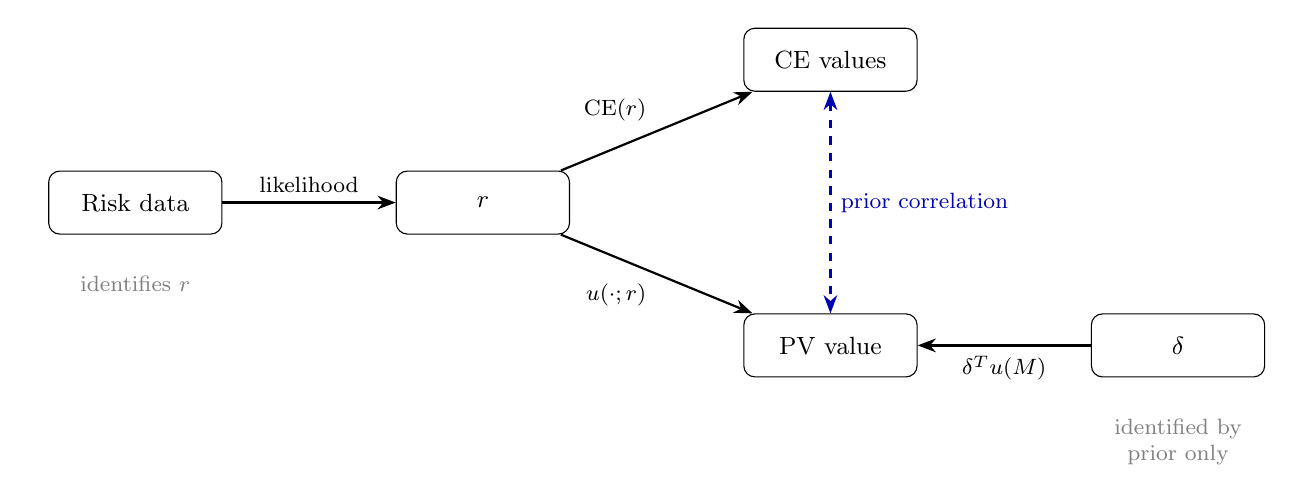
\begin{tikzpicture}[>=Stealth, node distance=2.2cm,
    box/.style={draw, rounded corners, minimum width=2.2cm,
                minimum height=0.8cm, align=center, font=\small}]

    % Nodes
    \node[box] (data) {Risk data};
    \node[box, right=of data] (r) {$r$};
    \node[box, above right=1cm and 2.2cm of r] (ce) {CE values};
    \node[box, below right=1cm and 2.2cm of r] (pv) {PV value};
    \node[box, right=of pv] (delta) {$\delta$};

    % Edges
    \draw[->, thick] (data) -- node[above, font=\footnotesize]
        {likelihood} (r);
    \draw[->, thick] (r) -- node[above left, font=\footnotesize]
        {$\CE(r)$} (ce);
    \draw[->, thick] (r) -- node[below left, font=\footnotesize]
        {$u(\cdot; r)$} (pv);
    \draw[->, thick] (delta) -- node[below, font=\footnotesize]
        {$\delta^T u(M)$} (pv);

    % Correlation
    \draw[<->, thick, dashed, blue!70!black]
        (ce) -- node[right, font=\footnotesize, text=blue!70!black]
        {prior correlation} (pv);

    % Annotations
    \node[below=0.4cm of data, font=\footnotesize, gray, text width=2.5cm,
          align=center] {identifies $r$};
    \node[below=0.4cm of delta, font=\footnotesize, gray, text width=2.5cm,
          align=center] {identified by\\prior only};
\end{tikzpicture}
\caption{%
    Information flow in the cross-domain prior. Risk data identify $r$
    through the likelihood. The CE values are determined by $r$. If the
    joint prior correlates CEs with PV (dashed blue arrow), the
    data-driven CEs indirectly constrain $\mathrm{PV}$, which in turn
    constrains $\delta$. Without this correlation, $\delta$ is identified
    only through the marginal PV prior conditional on $r$.
}
\label{fig:info_flow}
\end{figure}

This is standard Bayesian conditioning, but the observable-space formulation
makes the economic content transparent. The researcher can examine the
cross-domain correlation and ask: ``Do I really believe that knowing someone's
CEs tells me something about their discounting?'' If yes, the correlation
should be present. If not, use an independent prior and accept that $\delta$
is prior-driven.

\subsection{The General Principle}

The two cases above (disconnected and data-uninformed) illustrate a general
principle:

\begin{keyresult}[Cross-domain prior with partial data]
Let $\mathbf{Y} = (\mathbf{Y}_{\text{reach}}, \mathbf{Y}_{\text{unreach}})$
partition the observable quantities into those the model can compute and those
it cannot. Let $\btheta = (\btheta_{\text{id}}, \btheta_{\text{un}})$
partition the parameters into those identified by data and those that are not.
\begin{enumerate}
    \item \textbf{Unreachable quantities} ($\mathbf{Y}_{\text{unreach}}$):
    Marginalize out of the joint prior. Under independence, they vanish; under
    correlation, they shift the marginal prior on reachable quantities.

    \item \textbf{Unidentified parameters} ($\btheta_{\text{un}}$): The
    likelihood is flat in these parameters. The posterior is determined by
    the prior, with the data contributing indirectly through:
    \begin{itemize}
        \item The functional dependence of observables on both
        $\btheta_{\text{id}}$ and $\btheta_{\text{un}}$ (as in $\mathrm{PV}$
        depending on $r$), and
        \item Cross-correlations in the joint observable-space prior.
    \end{itemize}
\end{enumerate}
In all cases, the Gram determinant $\sqrt{\det(J^\top J)}$ accounts correctly
for the geometry. The framework is mathematically sound regardless of which
parameters are identified and which observables are reachable.
\end{keyresult}

\subsection{The BHM Extension: Hierarchical Cross-Domain Transmission}
\label{sec:bhm_cross}

In a Bayesian Hierarchical Model, the cross-domain prior channel becomes
richer. Consider $N$ subjects, each with parameters
$(r_i, \delta_i)$, and a population distribution on $(\CE, \mathrm{PV})$
jointly. Even if \emph{no individual subject} has time preference data:

\begin{enumerate}
    \item The risk data across all $N$ subjects update the population
    distribution of CEs (mean, variance, and --- if modeled ---
    higher moments).

    \item The population-level correlation between CE and PV transmits this
    update to the PV margin.

    \item Each subject's $\delta_i$ is informed by:
    \begin{itemize}
        \item Their own $r_i$ (through the conditional PV prior given $r_i$),
        \item The population-level CE--PV correlation (learned from all
        subjects' risk data).
    \end{itemize}
\end{enumerate}

This is a form of ``borrowing strength'' across economic domains rather than
across subjects. The hierarchical structure amplifies the prior correlation
channel: even a weak individual-level correlation becomes informative when
reinforced by $N$ subjects' worth of risk data constraining the population
CE distribution.

\begin{remark}[Transparency about identification]
It is essential to be transparent about which parameters are identified by data
and which are prior-driven. When reporting posterior estimates of $\delta$ from
a risk-only dataset, the researcher should clearly state that these estimates
reflect prior beliefs about the CE--PV relationship, not direct evidence from
time-preference data. The observable-space formulation makes this easier to
communicate than parameter-space priors: ``the posterior on discounting is
driven by our prior belief that risk aversion and patience are correlated''
is more interpretable than ``the posterior on $\delta$ reflects the prior
on $\delta$.''
\end{remark}

\subsection{Practical Implications}

The cross-domain framework has several practical implications:

\begin{enumerate}
    \item \textbf{Modular prior construction.} A researcher can build a joint
    prior over economic observables incrementally --- adding CEs, PVs, WTP
    measures, and other quantities as they are elicited. Each new domain
    extends $\mathbf{Y}$ with additional components.

    \item \textbf{Graceful degradation.} When a model or dataset addresses
    only a subset of the prior's domains, the irrelevant dimensions either
    drop out (disconnected case) or provide weak regularization through
    cross-correlations (data-uninformed case). The prior never breaks the
    model.

    \item \textbf{No wasted elicitation.} Prior beliefs about discounting are
    not ``wasted'' when applied to a risk-only model. If the researcher later
    adds time-preference data or a richer model, the same joint prior applies
    without modification, and the previously prior-driven $\delta$ estimates
    will be updated by the new data.

    \item \textbf{Sensitivity analysis.} The cross-correlation structure is
    a researcher degree of freedom. One should vary the correlation between
    domains and report how much the prior-driven parameters change. If the
    posterior on $\delta$ is highly sensitive to the CE--PV correlation, this
    signals that the data are uninformative about discounting and the
    results are prior-dependent.
\end{enumerate}

\begin{remark}[The three regimes]
The following table summarizes the three cases:
\begin{center}
\begin{tabular}{llll}
\toprule
Case & Jacobian rows & Likelihood & Effect of prior \\
\midrule
Fully informed & non-zero & depends on $\btheta$ & data + prior \\
Data-uninformed & non-zero & flat in some $\theta_j$ &
    prior-mediated \\
Disconnected & absent & N/A & marginalizes out \\
\bottomrule
\end{tabular}
\end{center}
The Gram determinant handles all three cases correctly. The mathematical
machinery does not distinguish between them --- the distinction is entirely
about which terms in the posterior are doing the work.
\end{remark}


%==============================================================================
\section{Normalization}
\label{sec:normalization}
%==============================================================================

\subsection{Is the Induced Prior Proper?}

Even if $p_{\mathbf{Y}}$ is a proper (normalized) density on $\mathbb{R}^n$,
the induced prior $p_{\btheta}$ need not integrate to 1 over $\mathbb{R}^k$.
This is because $p_{\btheta}$ concentrates the CE-space density onto a
$k$-dimensional manifold, and the ``total mass'' of $p_{\mathbf{Y}}$ along
this manifold depends on the manifold's geometry.

Formally:
\begin{equation}
    \int_{\mathbb{R}^k} p_{\btheta}(\btheta) \, d\btheta
    = \int_{\mathcal{M}} p_{\mathbf{Y}}(\mathbf{y}) \, d\sigma(\mathbf{y})
\end{equation}
This is the integral of $p_{\mathbf{Y}}$ over the manifold $\mathcal{M}$
with respect to its intrinsic surface measure. For a proper density
$p_{\mathbf{Y}}$, this integral is strictly less than 1 (since $\mathcal{M}$
has zero $n$-dimensional Lebesgue measure). But it is finite and positive as
long as $\mathcal{M}$ passes through a region where $p_{\mathbf{Y}} > 0$.

\subsection{Why This Is Fine for Bayesian Inference}

In Bayesian MCMC, the posterior is:
\begin{equation}
    p(\btheta \given \text{data}) \propto p(\text{data} \given \btheta) \,
    p_{\btheta}(\btheta)
\end{equation}

The proportionality constant (the marginal likelihood) absorbs any
normalization of the prior. For MCMC sampling, we only need $p_{\btheta}$ up
to a multiplicative constant, so unnormalized is fine.

For Bayes factors, the normalization does matter, and it is automatically
handled: the marginal likelihood integral includes the prior normalization.
A model whose manifold $\mathcal{M}$ passes through a low-density region of
$p_{\mathbf{Y}}$ will have a smaller marginal likelihood, all else equal.
This is exactly the Occam's razor discussed above.

\subsection{Sufficient Conditions for Properness}

The induced prior $p_{\btheta}$ is proper (finite integral) if:
\begin{enumerate}
    \item $p_{\mathbf{Y}}$ has light tails (e.g., Gaussian), and
    \item $\|\mathbf{g}(\btheta)\| \to \infty$ as $\|\btheta\| \to \infty$
    (the manifold escapes to infinity in CE space), and
    \item $\sqrt{\det(J^\top J)}$ grows at most polynomially.
\end{enumerate}
These conditions are easily satisfied for CE mappings of standard utility
functions: CEs are bounded by the prize range, so as $\|\btheta\| \to
\infty$, $\mathbf{g}(\btheta)$ approaches the boundary of the prize range,
where the Gaussian $p_{\mathbf{Y}}$ decays to zero.


%==============================================================================
\section{Injectivity in the Over-Determined Case}
\label{sec:injectivity}
%==============================================================================

The companion note discussed injectivity at length for the square case.
The over-determined case is \emph{strictly easier}.

\subsection{Why Over-Determination Helps}

For a square map $\mathbf{g}: \mathbb{R}^k \to \mathbb{R}^k$, injectivity
requires that distinct parameter vectors produce distinct CE vectors. When
$k < n$, we have \emph{more} constraints (CEs) than degrees of freedom
(parameters). This makes injectivity easier to achieve:

\begin{proposition}
\label{prop:over_inject}
If $\mathbf{g}: \mathbb{R}^k \to \mathbb{R}^n$ with $k < n$ has the property
that any $k$ components of $\mathbf{g}$ form an injective mapping, then
$\mathbf{g}$ itself is injective.
\end{proposition}

\begin{proof}
If $\mathbf{g}(\btheta) = \mathbf{g}(\btheta')$, then in particular the $k$
chosen components agree: $g_{i_1}(\btheta) = g_{i_1}(\btheta'), \ldots,
g_{i_k}(\btheta) = g_{i_k}(\btheta')$. By injectivity of the $k$-component
sub-mapping, $\btheta = \btheta'$.
\end{proof}

This is weaker than requiring \emph{all} $k$-component subsets to be
injective; any single subset suffices. The remaining $n - k$ CEs provide
redundant constraints that can only help.

\subsection{Rank Condition}

For the Gram determinant to be nonzero (so the area element is positive), the
Jacobian $J$ must have rank $k$. Since $J$ is $n \times k$ with $n > k$, this
requires that the $k$ columns of $J$ are linearly independent --- a weaker
condition than $\det J \neq 0$ for a square matrix (which requires $n = k$).

Geometrically, rank $k$ means the mapping is an immersion: it doesn't
collapse the parameter space to a lower-dimensional surface. For economic CE
mappings, this holds as long as the parameters have distinct effects on
at least one CE --- which is the identifying condition for the utility model.


%==============================================================================
\section{The General Table}
\label{sec:table}
%==============================================================================

\begin{center}
\begin{tabular}{ccccc}
\toprule
$k$ & $n$ & $J$ shape & Correction factor & Name \\
\midrule
$k = n$ & --- & $k \times k$ & $|\!\det J|$ & Standard Jacobian \\
$k < n$ & --- & $n \times k$ & $\sqrt{\det(J^\top J)}$ & Gram/area element \\
$k = 1$ & $n = 1$ & scalar & $|g'(r)|$ & Companion note \\
$k = 1$ & $n \geq 2$ & $n \times 1$ & $\|\nabla g(r)\|$ & Curve speed \\
\bottomrule
\end{tabular}
\end{center}

All cases are subsumed by the single formula
$\sqrt{\det(J^\top J)}$. The square-matrix determinant and the
1D absolute derivative are special cases.


%==============================================================================
\section{Practical Guidance}
\label{sec:practical}
%==============================================================================

\subsection{How Many CEs?}

The minimum is $n = k$ (square case): one CE per parameter. Additional CEs
($n > k$) provide:
\begin{enumerate}
    \item \textbf{Over-identification:} Multiple CE constraints anchor the
    prior more robustly.
    \item \textbf{Model agnosticism:} The same prior works for models with
    fewer parameters.
    \item \textbf{Bayes factor comparability:} Fair model comparison via
    shared priors.
\end{enumerate}

The cost is that each additional CE adds a row to $J$ and a term to the
CE-space prior. The computational overhead is minimal: computing $J^\top J$
and its determinant for small $k$ is cheap even if $n$ is moderately large.

\subsection{Choosing Reference Lotteries}

The reference lotteries should be chosen to ensure:
\begin{enumerate}
    \item \textbf{Rank condition:} $\text{rank}\, J = k$ at all parameter
    values in the prior support. This requires that the lotteries have
    sufficiently diverse probability structures.
    \item \textbf{Injectivity:} Some $k$-subset of the $n$ CEs forms an
    injective mapping (Proposition~\ref{prop:over_inject}).
    \item \textbf{Interpretability:} The researcher can state meaningful
    beliefs about each CE.
\end{enumerate}

\subsection{On the Log Scale for MCMC}

The log-posterior contribution from the CE-space prior is:
\begin{equation}
    \log p_{\btheta}(\btheta) = \log p_{\mathbf{Y}}\!\big(\mathbf{g}(\btheta)\big)
    + \frac{1}{2} \log \det\!\big(J^\top J\big)
\end{equation}

In JAX:
\begin{verbatim}
    J = jax.jacfwd(g)(theta)           # (n, k) Jacobian
    gram = J.T @ J                      # (k, k) Gram matrix
    sign, logdet = jnp.linalg.slogdet(gram)
    log_area_element = 0.5 * logdet     # Note: sign is always +1
                                        # since J^T J is PSD
\end{verbatim}

Note that $J^\top J$ is positive semi-definite by construction, so its
determinant is always non-negative. The sign from \texttt{slogdet} is always
$+1$ when $\text{rank}\, J = k$.

\subsection{Extension to the BHM}

The hierarchical extension from Section 6 of the companion note carries over
directly. Replace $|\!\det J_{\mathbf{g}}(\btheta_i)|$ with
$\sqrt{\det(J_{\mathbf{g}}(\btheta_i)^\top J_{\mathbf{g}}(\btheta_i))}$
in the per-subject prior term. The hyperprior on CE population means and
variances is unchanged.


%==============================================================================
\section{Relationship to the Coarea Formula}
\label{sec:coarea}
%==============================================================================

The mathematical foundation of the pullback measure is the \emph{area formula}
from geometric measure theory, which generalizes the change-of-variables
formula to maps between spaces of different dimensions.

\subsection{The Area Formula}

For a Lipschitz map $\mathbf{g}: \mathbb{R}^k \to \mathbb{R}^n$ ($k \leq n$)
and a non-negative measurable function $h: \mathbb{R}^k \to [0, \infty)$:
\begin{equation}
    \int_{\mathbb{R}^k} h(\btheta) \,
    \underbrace{\sqrt{\det\!\big(J_{\mathbf{g}}^\top J_{\mathbf{g}}\big)}}_{
    \text{Jacobian multiplier}} \, d\btheta
    = \int_{\mathbb{R}^n}
    \underbrace{\sum_{\btheta \in \mathbf{g}^{-1}(\mathbf{y})}
    h(\btheta)}_{\text{sum over preimages}} \;
    d\mathcal{H}^k(\mathbf{y})
\end{equation}
where $\mathcal{H}^k$ is the $k$-dimensional Hausdorff measure.

When $\mathbf{g}$ is injective, each fiber $\mathbf{g}^{-1}(\mathbf{y})$
has at most one element, and the right side becomes an integral over the
image manifold $\mathcal{M}$. Taking
$h(\btheta) = p_{\mathbf{Y}}(\mathbf{g}(\btheta))$ and using the
definition of the pullback measure recovers our formula.

\subsection{Connection to the Standard Change of Variables}

When $k = n$, the Hausdorff measure $\mathcal{H}^n$ coincides with
$n$-dimensional Lebesgue measure, $\sqrt{\det(J^\top J)} = |\!\det J|$, and
the area formula reduces to the standard substitution rule for integrals.

The over-determined case ($k < n$) is a genuine generalization: the target
measure is no longer Lebesgue on $\mathbb{R}^n$ but Hausdorff on the
embedded manifold. The Gram determinant is the correct volume element for
this lower-dimensional integration.


%==============================================================================
\section{Summary}
\label{sec:summary}
%==============================================================================

\begin{keyresult}[The three facts you need]
\begin{enumerate}
    \item \textbf{The formula generalizes.} When the CE mapping
    $\mathbf{g}: \mathbb{R}^k \to \mathbb{R}^n$ has more outputs ($n$) than
    inputs ($k$), the Jacobian correction $|\!\det J|$ is replaced by the Gram
    determinant $\sqrt{\det(J^\top J)}$, where $J$ is the $n \times k$
    Jacobian. For the square case ($k = n$), this reduces to $|\!\det J|$.

    \item \textbf{The computation is forward-only.} As in the square case,
    evaluating the pullback prior at a proposed $\btheta$ requires only the
    forward map $\mathbf{g}(\btheta)$ and its Jacobian. The Gram matrix
    $J^\top J$ is $k \times k$ (always square), and computing its determinant
    is cheap via autodiff + \texttt{slogdet}.

    \item \textbf{The prior is model-agnostic.} The same CE-space prior works
    for utility models of any dimensionality $k \leq n$. The model determines
    which manifold in CE space is reachable; the pullback measure restricts
    the CE prior to that manifold automatically. This enables fair Bayes
    factor comparisons and provides a natural Occam's razor.
\end{enumerate}
\end{keyresult}

\noindent
The over-determined CE prior is not a limitation or a special case requiring
separate treatment. It is the natural setting for model-agnostic prior
specification: state beliefs about observables, and let the model's
structure determine how those beliefs map to parameters. The Gram determinant
is the mathematical tool that makes this work.


\end{document}
